% !TeX root = planung.tex
\documentclass[fleqn]{../swp}
\usepackage{tikz-uml}

\textwidth 18.5cm
\textheight 25.5cm
\hoffset=-2.9cm
\voffset=-2.9cm

\sloppy
\hyphenpenalty 10000000

\begin{document}
        \fontfamily{arial}
        \sffamily
        \renewcommand\documentTitle{Anwendungsfälle Anhang UML Diagramme und weitere Detailbeschreibungen}
        \renewcommand\groupName{KarteikartenAG}
        \swpdocument{Rodrigue Wete Nguempnang}{13. November 2022}%
                    {Mert As & meras@uni-bremen.de}%
                    {Tom Beuke & tombeuke@uni-bremen.de}%
                    {Efe Carkcioglu & efe1@uni-bremen.de}%
                    {Nadja Cordes & ncordes@uni-bremen.de}%
                    {Ole-Niklas Mahlstädt & olma@uni-bremen.de}%
                    {Henry Zöllner & henry5@uni-bremen.de}%

        \newpage\large{Login UML Case Diagramm}

\newcommand{\servername}{KarteikartenAG Server}
\newcommand{\clientname}{User}
\newcommand{\systemname}{KarteikartenAG Client}

\begin{center}
    \begin{tikzpicture}
        \begin{umlsystem}[x=4, fill=red!10]{\systemname}
            \umlusecase[y=-2, name=login]{Login Page}
            \umlusecase[x=4, width=2.2cm, name=loginfailed]{Login Fehlgeschlagen}
        \end{umlsystem}

        % Actors
        \umlactor[y=-4]{User}
        \umlactor[x=12, y=-4]{\servername}

        % Login
        \umlassoc[geometry=|-]{\clientname}{login}
        \umlVHextend{loginfailed}{login}
        \umlassoc[name=loginserver, geometry=|-]{\servername}{login}
        \umlnote[x=8, y=-5]{loginserver-1}{TLS?}
    \end{tikzpicture}
\end{center}

\begin{answer}
    Die Loginseite ist das erste was der User sieht nachdem dieser das Programm zum ersten mal startet. \\
    Auf dieser hat er die Möglichkeit sich auf dem Karteikartenserver anzumelden. Falls der User noch keinen Account erstellt hat kann er dies auf der selben Seite tun. Der Server überprüft danach die Logindaten. Wenn diese nicht stimmen oder ein anderer Fehler entsteht wird eine ,,Login Fehlgeschlagen'' Nachricht an den User geschickt.

    
    \resizebox{210pt}{200pt}{
        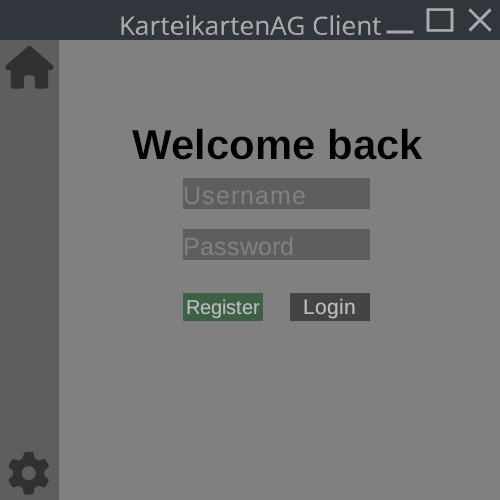
\includegraphics{images/login.jpg}
    } \\
    \noindent
    Von der Loginseite kann man ohne sich anzumelden \\ 
    bereits auf die Einstellungen zugreifen.

\end{answer}      % Tom
        \newpage\large{Einstellungen UML Case Diagramm}
\begin{center}
    \begin{tikzpicture}
        \begin{umlsystem}[x=4, fill=red!10]{\systemname}
            \umlusecase[y=-10, name=setting-0]{Settings}
            \umlusecase[x=5, y=-3.5, width=1.5cm, name=setting-1]{Sprache wählen}
            \umlusecase[x=10, y=-20, width=1.5cm, name=setting-2]{Check if already logged in}
            \umlusecase[x=5, y=-6, width=1.5cm, name=setting-3]{Exportiert Kategorie als PDF}
            \umlusecase[x=10, y=-5, width=1.5cm, name=setting-4]{Deutsch}
            \umlusecase[x=10, y=-3, width=1.5cm, name=setting-5]{Englisch}
            \umlusecase[x=5, y=-8.7, width=1.5cm, name=setting-6]{Exportiert Kategorie als JSON}
            \umlusecase[x=5, y=-11.5, width=1.5cm, name=setting-7]{Exportiert Kategorie als XML}
            \umlusecase[x=4, y=-18, width=1.5cm, name=setting-8]{Logout}
            \umlusecase[x=10, y=-7.5, width=1.5cm, name=setting-10]{Die aktuelle Kategorie}
            \umlusecase[x=10, y=-11, width=1.5cm, name=setting-11]{Eine andere Kategorie}
            \umlusecase[x=5, y=-14, width=1.5cm, name=setting-12]{Hellmodus}
            \umlusecase[x=5, y=-16, width=1.7cm, name=setting-13]{Dunkelmodus}
            \umlusecase[x=10, y=-14, width=1.7cm, name=setting-14]{Waehle eine Kategorie}
            
        \end{umlsystem}

        % Actors
        \umlactor[y=-6]{User}
        \umlactor[x=17, y=-6]{\servername}


        % Settings
        \umlassoc[geometry=|-]{\clientname}{setting-0}
        \umlextend{setting-1}{setting-0}
        
        \umlextend{setting-8}{setting-0}
        \umlVHinclude{setting-2}{setting-8}
        
        \umlextend{setting-4}{setting-1}
        \umlextend{setting-5}{setting-1}
        
        \umlassoc[geometry=|-]{\servername}{setting-8}
        
        \umlextend{setting-6}{setting-0}
        \umlextend{setting-7}{setting-0}
        \umlextend{setting-3}{setting-0}
        
        
        \umlextend{setting-12}{setting-0}
        \umlextend{setting-13}{setting-0}
        
        \umlextend{setting-10}{setting-3}
        \umlextend{setting-10}{setting-6}
        \umlextend{setting-10}{setting-7}
        
        \umlextend{setting-11}{setting-3}
        \umlextend{setting-11}{setting-6}
        \umlextend{setting-11}{setting-7}
        
        \umlinclude{setting-11}{setting-14}
        
    \end{tikzpicture}
\end{center}

\begin{answer}
    Detailanwendungsfall die Sprache auf Englisch umstellen 
\end{answer}
\newline
\textbf{Akteure}: Schüler Sam
\newline
\textbf{Vorbedingungen}: 
\begin{itemize}  
    \item Das System ist gestartet.
    \item Sam hat sich nicht gemeldet.
   \item Das System ist auf Deutsch.
\end{itemize} 
\textbf{Nachbedingungen}: 
\begin{itemize}  
    \item Er hat die App Sprache erfolgreich von Deutsch auf Englisch geändert.
   \item Oder, er kann nicht finden, wo man die Sprache ändern kann.\\
\end{itemize}
\textbf{Regulärer Ablauf}: 
\begin{itemize}  
    \item Sam klickt auf den Button Settings.
   \item Weitere Funktionen von Settings werden angezeigt. (siehe Abb.)
   \item Sam bringt sein Mauszeiger zu Sprachen.
    \item Weitere Funktionen von Sprachen werden angezeigt.
    \item Sam klickt auf den Button Englisch.
     \item Die Sprache wurde auf Englisch umgestellt.
\end{itemize}
\textbf{Alternative}: 
\begin{itemize}  
    \item Er hat nicht genug Deutschkentnisse, das Wort ,,Sprachen'' zu verstehen. Deswegen bringt er sein Mauszeiger nicht zu Sprachen und kann das Button ,,Englisch" nicht finden.
\end{itemize}    % Efe
        \newpage\large{Karteikarten UML Case Diagramm}
\begin{center}
    \begin{tikzpicture}
        \begin{umlsystem}[x=4, fill=red!10]{\systemname}
            \umlusecase[x=0, y=-6, width=1.5cm, name=createcard]{Neue Karte erstellen}
            \umlusecase[x=0, y=-12, width=1.5cm, name=editcard]{Karte bearbeiten}
	    \umlusecase[x=0, y=-17.0, width=1.5cm, name=deletecard]{Karte löschen}
            \umlusecase[x=5 	, y=-8, width=1.5cm, name=cardtype]{Kartentyp auswählen}
            \umlusecase[x=5 , y=-11.0, width=1.5cm, name=takeinput]{Karte Informationen nehmen}
            \umlusecase[x=5 , y=-13.0, width=1.5cm, name=tag]{Schlagwort hinzufügen}
	    \umlusecase[x=5 , y=-15.0, width=1.5cm, name=bewertung]{Karte bewerten}	
            \umlusecase[x=10, y=-5, width=1.5cm, name=multiplechoicetest]{Ankreuztest}
 	    \umlusecase[x=5, y=-5, width=1.5cm, name=kategorie]{Kategorie wählen}
            \umlusecase[x=10, y=-7, width=1.5cm, name=truefalsetest]{Wahr/Falsch Test}
            \umlusecase[x=10, y=-9, width=1.5cm, name=texttest]{Texteingabe Test}
	    \umlusecase[x=10, y=-11, width=2cm, name=imagetest]{Bild Test}
            \umlusecase[x=10, y=-13, width=2cm, name=3dtest]{Bildbeschreibung Test}
            \umlusecase[x=10, y=-15.0, width=1.5cm, name=audiotest]{Audio Test}

        \end{umlsystem}

        % Actors
        \umlactor[y=-6]{Benutzer}
        \umlactor[x=17.5, y=-6]{\servername}

        % Card Related
       %% \umlVHextend{editcard}{exportcard}

	\umlextend{tag}{createcard}
	\umlextend{tag}{editcard}
	\umlinclude{createcard}{cardtype}
        \umlinclude{createcard}{kategorie}
	\umlinclude{createcard}{takeinput}
	\umlextend{bewertung}{editcard}
        \umlextend{cardtype}{editcard}
	\umlextend{takeinput}{editcard}
        \umlinherit{cardtype}{multiplechoicetest}
        \umlinherit{cardtype}{truefalsetest}
        \umlinherit{cardtype}{texttest}
        \umlinherit{cardtype}{imagetest}
	\umlinherit{cardtype}{3dtest}
	\umlinherit{cardtype}{audiotest}
	\umlassoc[geometry=-|]{editcard}{\servername}
        \umlassoc[geometry=-|]{createcard}{\servername}
	\umlassoc[geometry=-|]{editcard}{User}
        \umlassoc[geometry=-|]{createcard}{User}
	\umlassoc[geometry=-|]{deletecard}{User}
	\umlassoc[geometry=-|]{deletecard}{\servername}

    \end{tikzpicture}
\end{center}



      % Mert
        \newpage\begin{center}
    \begin{tikzpicture}
        \begin{umlsystem}[x=4, fill=red!10]{\systemname}
            \umlusecase[x=0, y=-19, width=1.5cm, name=choosedecks]{choose deck(s)}
            	\umlusecase[x=4, y=-21, width=1.5cm, name=methodoftesting]{pick method of testing}
            		\umlusecase[x=2, y=-23, width=1.5cm, name=leitnersystem]{use leitner method}
            			\umlusecase[x=2, y=-25, width=1.5cm, name=sorting]{set order of cards}
            				\umlusecase[x=0, y=-27, width=1.5cm, name=alphabetical]{use alphabetical order}
            				\umlusecase[x=4, y=-27, width=1.5cm, name=random]{use random order}
            		\umlusecase[x=6, y=-23, width=1.5cm, name=othersystem]{use other method}
            \umlusecase[x=6, y=-19, width=1.5cm, name=starttest]{start test}
            \umlusecase[x=10, y=-19, width=1.5cm, name=checktest]{check test}
            %\umlusecase[x=6, fill=green!20]{use case5}
            %\umlusecase[x=6, y=-4]{use case6}
        \end{umlsystem}

        % Actors
        \umlactor[y=-16]{User}
        \umlactor[x=17.5, y=-16]{\servername}


        % Tests
        \umlassoc[geometry=|-]{\clientname}{choosedecks}
		\umlassoc{choosedecks}{methodoftesting}
		\umlassoc{methodoftesting}{starttest}
		\umlinherit{leitnersystem}{methodoftesting}
		\umlassoc{sorting}{leitnersystem}
		\umlinherit{alphabetical}{sorting}
		\umlinherit{random}{sorting}
		\umlinherit{othersystem}{methodoftesting}
		\umlextend{starttest}{checktest}
        \umlassoc[geometry=-|]{checktest}{\servername}
    \end{tikzpicture}
\end{center}

    % Henry
        \newpage\large{Kategorien UML Case Diagramm}
\begin{center}
    \begin{tikzpicture}
        \begin{umlsystem}[x=4, fill=red!10]{\systemname}
            \umlusecase[x=6, y=-1.5, width=2.5cm, name=edit]{Kategorie bearbeiten}
            \umlusecase[x=10, y=0, width=2.5cm, name=name]{Name setzen}
            \umlusecase[x=10, y=-3, width=2.5cm, name=poly]{Polyhierarchie definieren}
            \umlusecase[x=2, y=-3.5, name=create]{Kategorie anlegen}
			\umlusecase[x=4, y=-4.5, name=delete]{Kategorie löschen}
			\umlusecase[x=0, y=-10, name=overview]{Übersicht}
			\umlusecase[x=5, y=-9, name=sort]{Übersicht sortieren}
			\umlusecase[x=5, y=-11, name=view]{Polyhierarchie ansehen}
			\umlusecase[x=7, y=-10, name=select]{mehrere Kategorien auswählen}
			\umlusecase[x=10, y=-8, width=2.5cm,name=action]{Aktion über Kategorieauswahl}
			
			\umlusecase[x=6, y=-6.5, width=2.5cm,name=export]{Export als PDF/JSON/XML}
			\umlusecase[x=11, y=-6, width=2cm,name=deck]{Karteikasten erstellen}
        \end{umlsystem}

        % Actors
        \umlactor[y=-6]{User}
        
        % Associations
        \umlassoc[geometry=|-]{User}{edit}
        \umlinherit{name}{edit}
        \umlinherit{poly}{edit}
        \umlextend{create}{edit}
        \umlextend{delete}{edit}
        \umlassoc[geometry=|-]{User}{overview}
		\umlinclude{overview}{sort}
		\umlassoc{overview}{select}
		\umlassoc{overview}{view}
        \umlassoc{select}{action}
        \umlextend{action}{edit}
        \umlinclude{action}{export}
        \umlinclude{action}{deck}
    \end{tikzpicture}
\end{center}

 % Ole
        \newpage
\large{Glossar UML Case Diagramm}

\begin{center}
    \begin{tikzpicture}
        \begin{umlsystem}[x=4, fill=red!10]{\systemname}
            \umlusecase[y=-10, x= 7, name=overviewcards]{Overview Cards}
            \umlusecase[y=-8.5, x=10, name=sorting]{Alphabetical sorting}
            \umlusecase[y=-14, x=9, name=filtering]{Filter function}
            \umlusecase[y=-14.5, x=1.5,  name=dSorting]{Sorting function}
            \umlusecase[y=-15.5, x=5,  name=hide]{(Un)hide function}
            \umlusecase[y=-13.5, x=0,  name=display]{Display columns}
            \umlusecase[y=-11.5, x=-1,  name=colType]{Type}
            \umlusecase[y=-12, x=1,  name=colCreatedAt]{CreatedAt}
            \umlusecase[y=-11, x=2.5,  name=colQuestion]{Question}
            \umlusecase[y=-12.5, x=-1,  name=colAnswer]{Answer}
            \umlusecase[y=-10.5, x=0.5,  name=colCntDecks]{Count of Decks}
            \umlusecase[y=-15,x=10,  name=filterCategories]{Categories}
            \umlusecase[y=-12.5,x=10, name=filterWords]{Tags}
            \umlusecase[y=-13,x=8,  name=filterSearchWords]{Search words}
            \umlusecase[y=-19, x=-1,  name=showCard]{Show card}
            \umlusecase[y=-21, x=8,  name=selectCard]{Do (Multi)select}
            
              \umlusecase[y=-22, x=8,  name=cardActions1]{Edit/Delete Card(s)}
            \umlusecase[y=-19.5, x=7,  name=cardActions2]{Create Card}
             \end{umlsystem}

        % Actors
        \umlactor[y=-6]{User}
        \umlactor[x=17.5, y=-6]{\servername}

        % Card Related
    \umlassoc[geometry=|-]{\clientname}{overviewcards}
    \umlassoc[geometry=|-]{\servername}{overviewcards}
    \umlextend{filtering}{overviewcards}
    \umlinclude{overviewcards}{sorting}
    \umlinclude{overviewcards}{display}
    \umlinherit{colType}{display}
    \umlinherit{colAnswer}{display}
    \umlinherit{colCntDecks}{display}
    \umlinherit{colQuestion}{display}
    \umlinherit{colCreatedAt}{display}
    \umlextend{selectCard}{overviewcards}
    \umlextend{hide}{overviewcards}
    \umlinherit{filterCategories}{filtering}
    \umlinherit{filterWords}{filtering}
    \umlinherit{filterSearchWords}{filtering}
    \umlassoc{cardActions1}{selectCard}
    \umlextend{showCard}{overviewcards}
    \umlextend{dSorting}{overviewcards}
    \umlextend{cardActions2}{overviewcards}
    \umlassoc[geometry=|-]{\clientname}{cardActions1}
    \umlassoc[geometry=|-]{\clientname}{cardActions2}
    \umlassoc[geometry=|-]{\clientname}{showCard}
   
    \end{tikzpicture}
\end{center}
      

\begin{answer}
    Detailanwendungsfall Einzelkartenansicht 
\end{answer}
\newline
\textbf{Akteure}: Lehrer Leo, (Studi Susi)
\newline
\textbf{Vorbedingungen}: 
\begin{itemize}  
    \item Das System ist gestartet.
    \item Leo ist angemeldet und möchte seine bereits erstellten Karteikarten einsehen. 
    Er glaubt, dass er sich bei der Karteikarte \dq Bundesländer Deutschland\dq bei der Antwort vertippt hat und möchte diese nachträglich einsehen und ggfs. anpassen, bevor er dazu einen Karteikasten für seinen Schüler Sam erstellt.
\end{itemize} 
\vspace{0,2cm}
\textbf{Nachbedingungen}: 
\begin{itemize}  
    \item Die Karte ist in der Detailansicht geöffnet.
    \item Oder: Karte ist nicht vorhanden
\end{itemize}
\vspace{0,5cm}
\textbf{Regulärer Ablauf}: 
\begin{enumerate}  
    \item Leo öffnet sein Karteikartenglossar.

        \begin{center}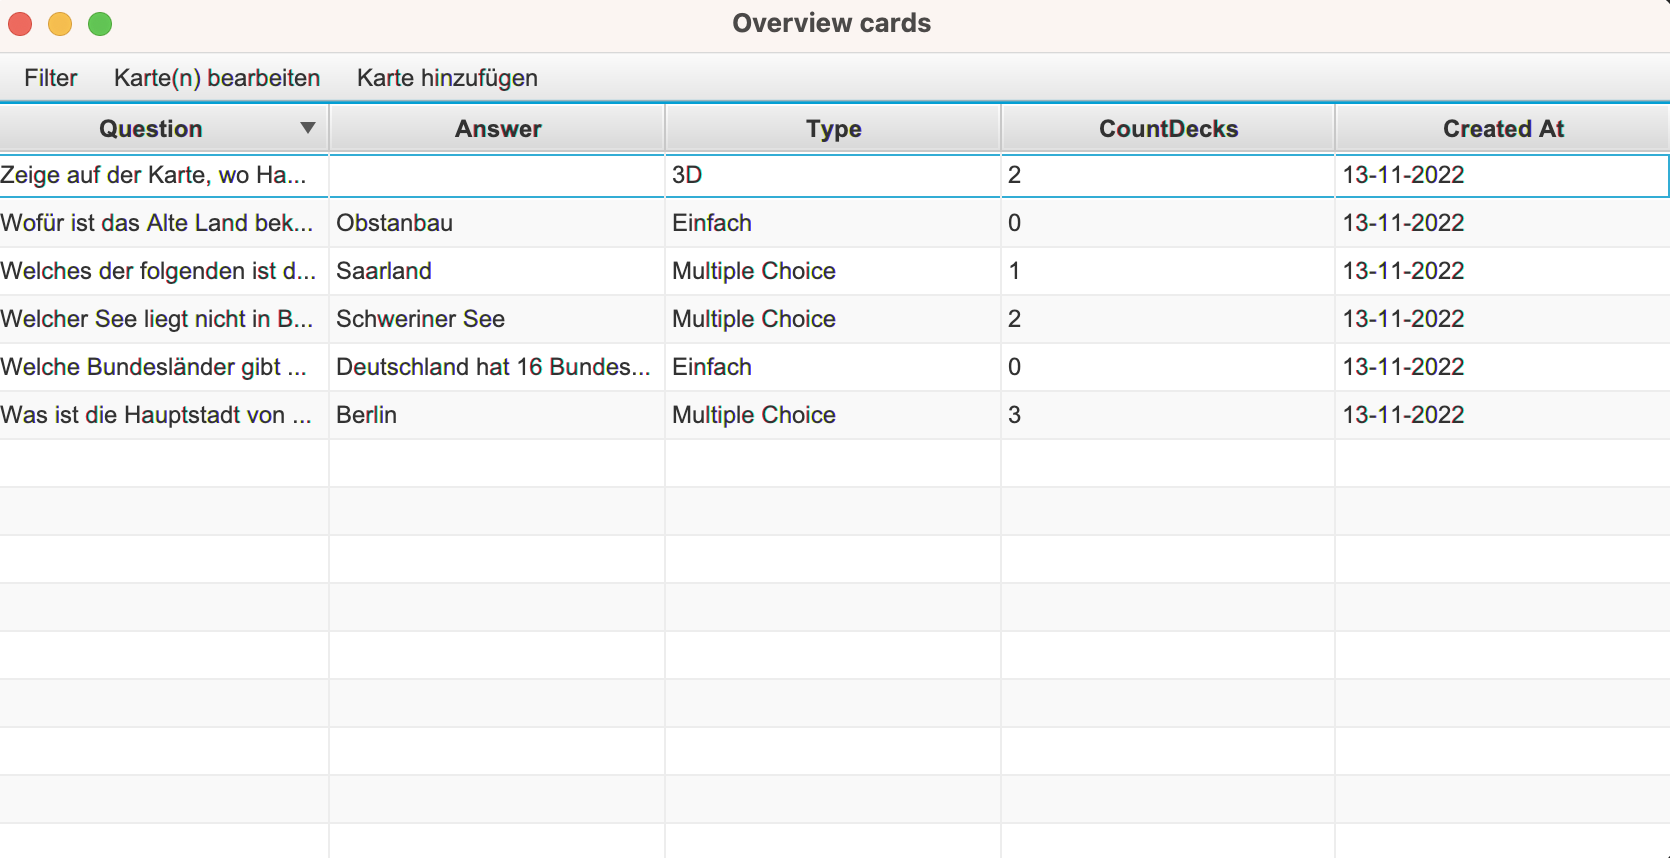
\includegraphics[width=17cm,height=35cm,keepaspectratio]{images/overview-details1.png}\end{center} 
       
    \item Er scrollt durch sein Glossar und sucht nach der Karte.
    \item Er entdeckt die gewünschte Karte und markiert sie.
    \item Er klickt auf den Button \dq Einzelkartenansicht\dq.
    \begin{center}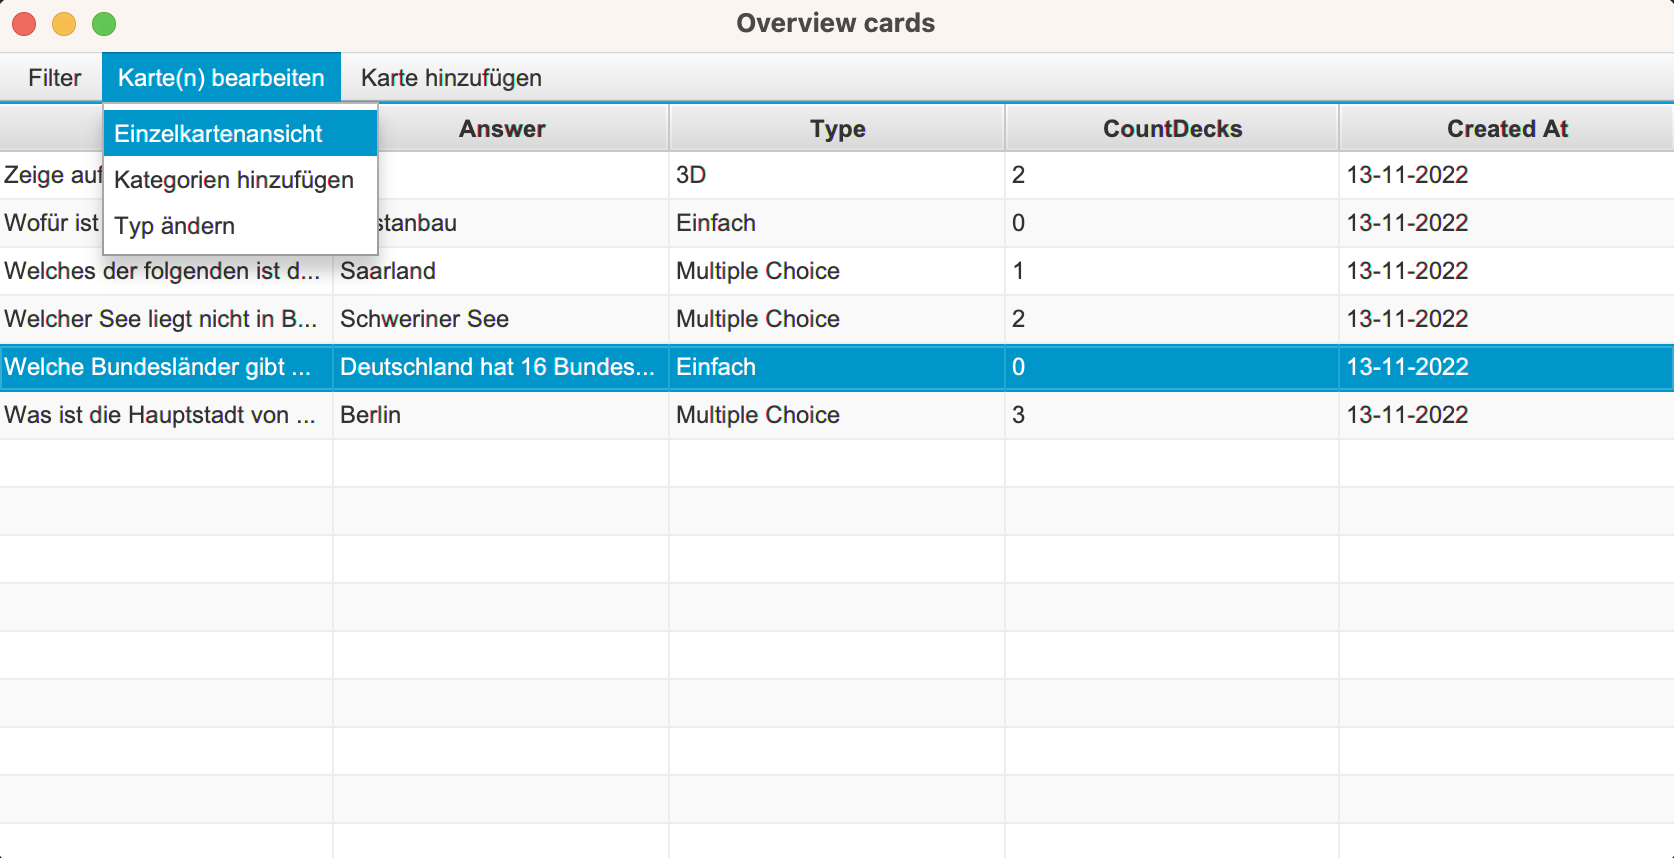
\includegraphics[width=17cm,height=35cm,keepaspectratio]{images/overview-details2.png}\end{center} 
    
    \item Er kann die Karte samt Details in einem neuen Fenster einsehen und bekommt dort alle Bearbeitungsoptionen der Karten zur Auswahl.
    \begin{center}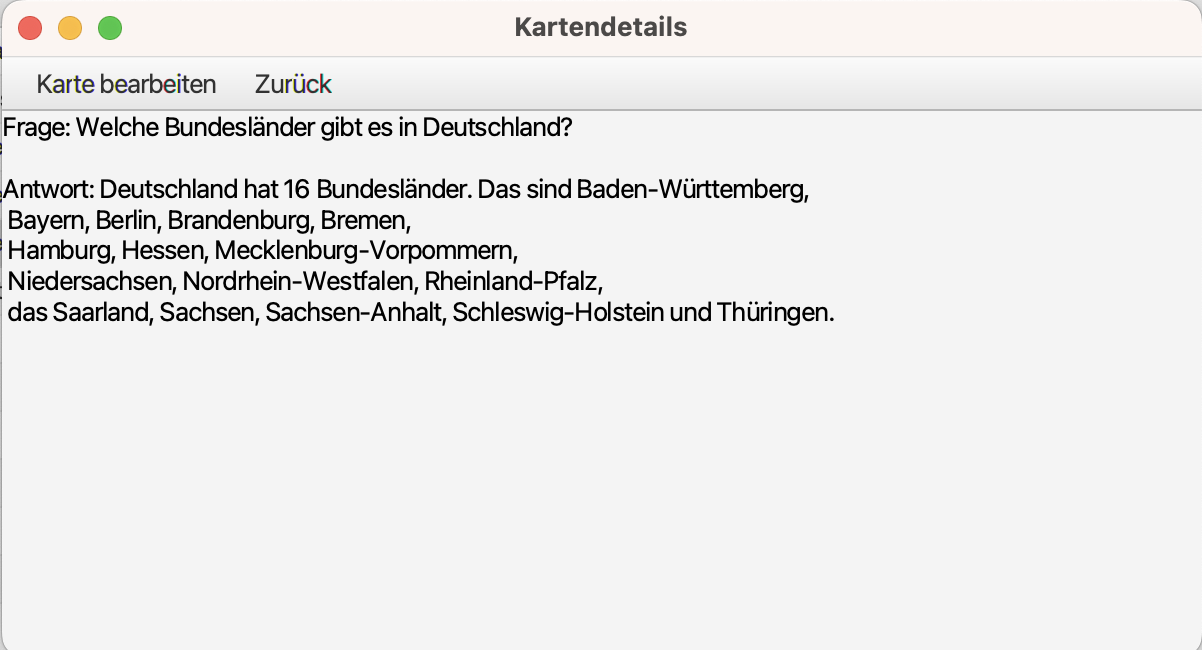
\includegraphics[width=17cm,height=35cm,keepaspectratio]{images/overview-details3.png}\end{center} 
       
\end{enumerate} 
\textbf{Alternative}:
\newline Zu 3. Da er die Karte auf Anhieb nicht findet, filtert er durch die Suchwörter mittels Eingabe von \dq Bundesländer Deutschland\dq nach der gewünschten Karte.
\newline Zu 3. Die gewünschte Karte existiert nicht. Leo legt stattdessen eine neue über den Button \dq Karte anlegen\dq an.
   % Nadja
        \newpage\large{Decks UML Case Diagramm}

\begin{center}
    \begin{tikzpicture}
        \begin{umlsystem}[x=4, fill=red!10]{\systemname}
        	\umlusecase[x=0, y=-2, name=overview]{Übersicht}
        	\umlusecase[x=0, y=-12, width=2cm, name=edit]{Karteikasten bearbeiten}
        	\umlusecase[x=6, y=-11, width=2cm, name=create]{Karteikasten erstellen}
        	\umlusecase[x=6, y=-13, width=2cm, name=delete]{Karteikasten löschen}
        	\umlusecase[x=0, y=-8.5, width=1.6cm, name=order]{Reihenfolge der Karten}
        	\umlusecase[x=2, y=-10, width=1.5cm, name=system]{Lernsystem wählen}
        	\umlusecase[x=5, y=-3, width=1.8cm, name=progress]{Lernfortschritt angucken}
        	\umlusecase[x=5, y=-4.5, width=2cm, name=poly]{Polyhierarchie angucken}
        	\umlusecase[x=1.8, y=-4.5, name=sort]{sortieren}
        	\umlusecase[x=-0.5, y=-3.75, name=filter]{filtern}
        	\umlusecase[x=1, y=-6, width=2cm, name=select]{einen/mehrere auswählen}
        	\umlusecase[x=5, y=-7.5, width=2cm, name=testing]{Lernvorgang starten}
        	\umlusecase[x=6, y=-6, width=2cm, name=export]{Export PDF/JSON/XML}
        	\umlusecase[x=6, y=-9, width=2cm, name=privpub]{privat/öffentlich stellen}
        \end{umlsystem}

        % Actors
        \umlactor[y=-8]{user}
        \umlactor[x=14, y=-8]{server}
        
        % Associations
        \umlassoc[geometry=|-]{user}{edit}
        \umlassoc[geometry=|-]{user}{overview}
        \umlextend{create}{edit}
        \umlextend{delete}{edit}
        \umlextend{privpub}{edit}
        \umlextend{order}{edit}
        \umlextend{system}{edit}
        \umlextend{filter}{overview}
        \umlextend{sort}{overview}
        \umlassoc{select}{overview}
        \umlinclude{select}{edit}
        \umlinclude{select}{testing}
        \umlinclude{select}{export}
        \umlassoc{progress}{overview}
        \umlassoc{poly}{overview}
        \umlassoc{server}{privpub}
        
    \end{tikzpicture}
\end{center}

      % Ole
        \newpage\large{Server UML Case Diagramm}
\begin{center}
    \begin{tikzpicture}
        \begin{umlsystem}[x=4, fill=red!10]{\systemname}
        	\umlusecase[x=0,   y=-4,   width=2.8cm, name=config]{Konfigurationsdatei}
        	\umlusecase[x=5,   y=-3,   width=1.8cm, name=port]{Port ändern}
        	\umlusecase[x=5,   y=-4.5, width=2cm,   name=prefix]{Präfix ändern}
        	\umlusecase[x=5.5, y=-6.5, width=2cm,   name=attempts]{Anzahl Loginversuche ändern}
        	\umlusecase[x=2,   y=-7,   width=2cm,   name=timeout]{Login timeout ändern}
        	\umlusecase[x=-1,  y=-6,   width=2cm,   name=manual]{Manuelles Registrieren erlauben}

        	\umlusecase[x=0, y=-11, width=2cm,   name=tool]{Datenbank Tool}
        	\umlusecase[x=6, y=-11, width=2.5cm, name=create]{Datenbankeintrag erstellen}
        	\umlusecase[x=6, y=-13, width=2.5cm, name=delete]{Datenbankeintrag löschen}
        	\umlusecase[x=6, y=-9,  width=2.5cm, name=edit]{Datenbankeintrag ändern}
        \end{umlsystem}

        % Actors
        \umlactor[y=-8]{Admin}
        
        % Associations
        \umlassoc[geometry=|-]{Admin}{tool}
        \umlinclude{create}{tool}
        \umlinclude{delete}{tool}
        \umlinclude{edit}{tool}

        \umlassoc[geometry=|-]{Admin}{config}
        \umlextend{port}{config}
        \umlextend{prefix}{config}
        \umlextend{attempts}{config}
        \umlextend{timeout}{config}
        \umlextend{manual}{config}
        
    \end{tikzpicture}
\end{center}

     % Tom
\end{document}